\chapter{Introduction}
Analysis of electrical machines is a very well-known subject in electrical engineering and at a first glance one might think that this field cannot be embarked on any further. However, this is not the case, since advances in materials such as permanent magnets offer new possibilities which might not have been economical a few years ago. In addition to the development of the materials used in electrical machines, the mathematical and physics software tools for solving complex problems and the visualisation of the results have also improved. Furthermore, the technologies driving the microprocessors and storage devices used in personal computers have contributed to solve difficult mathematical functions by means of numerical methods. All these factors have influenced the way electrical machines are designed and will be designed in the future. The research presented in this book is a typical example of how advances in other fields can lead to new ideas in electrical engineering, and especially electrical machines. 
\index{microprocessors}
\index{storage devices}

\section{Problem statement}
\label{sec:problem_statement}
Designing the winding is from an electromagnetic point of view the most important part in machine design. In this step the coil sides of the phases need to be assigned to an appropriate stator slot which allows a rotating magnetic field when phase displaced currents are applied to the winding. Once the assignment is done, adjacent coil sides belonging to the same phase are called a phase belt. This is the definition used in modern textbooks such as that written by \cite{REF-00330} and was already in use in early papers by \cite{REF-00835, REF-00836}.

In order to design symmetrical windings, it is necessary to have a systematic algorithm to allocate the slots. Then, after doing this, the coils can be inserted in the appropriate slots. The immediate and essential main question that first needs to be answered is: 
\begin{quote}
\textbf{What is the mathematical expression to allocate the stator slots belonging to a phase belt?} 
\end{quote}

Another sub-question arises from the requirement to allocate the slots that belong to a phase belt. Especially when using FEM to analyse machines, the entering of the winding arrangement is a complex process. The problem is exacerbated if different winding types are to be analysed. Furthermore, in the conceptual design phase a compact representation of the winding could simplify the choice of the initial geometrical parameters. Therefore the sub-question is: 
\begin{quote}
\textbf{How can a winding layout be represented in a compact form?} 
\end{quote}
\index{conceptual design phase}

\section{Overlapping and non-overlapping windings}\label{sec:def_con}  
Fig.~\ref{fig:flux_coils}\subref{fig:dow} shows a double layer overlapping winding. In the drawing some of the coils are removed which makes it easier to identify the two layers. A non-overlapping single layer winding is shown in Fig.~\ref{fig:flux_coils}\subref{fig:snow}. Only each second stator tooth has a coil wound around it. 
\begin{figure}[htbp]
  \fontsize{6}{8}\selectfont
  \centering
  \subfloat[Overlapping winding\label{fig:dow}]{
  \begin{overpic}[scale=0.55]
  {figs/DOW.eps}
  \put(20,10){\vector(1,1){12}}
  \put(5,7){double layer coil}
  \end{overpic}}
  \hfill
  \subfloat[Non-overlapping\label{fig:snow}]{
  \begin{overpic}[scale=0.55]
  {figs/SNOW.eps}
  \put(12,10){\vector(1,1){12}}
  \put(5,7){single layer coil}
  \put(50,40){\vector(-2,-1){14}}
  \put(45,41){stator tooth}
  \end{overpic}}
  \caption{Double layer overlapping and single layer non-overlapping windings}
  \label{fig:flux_coils}
\end{figure}
\index{overlapping}
\index{non-overlapping}

Non-overlapping windings are a sub-set of fractional slot windings and need some extra discussion. It is often categorised as concentrated. This is not necessarily wrong but is incongruent with the formal definition. The opposite of a concentrated winding is a distributed winding. In the latter case a the coils of a given phase are distributed in several slots. When referring to overlapping and non-overlapping windings a concentrated winding could be defined as follows:
\begin{enumerate}
  \item Formally a concentrated winding is one where the number of slots per pole and~%
  phase equals one. In this case the coil pitch equals the pole pitch and it is~%
  categorised as overlapping. This means that each coil side of the winding is~%
  placed in a single slot. If the coil spans a pole pitch, it is called a full-pitch~%
  concentrated winding.
  \item Non-overlapping could also be classified as concentrated, but then it is not~%
  done in terms of the formal definition. Concentrated in this case means that a coil~%
  is concentrated around a stator tooth as shown in Fig.~\ref{fig:flux_coils}\subref{fig:snow}.
\end{enumerate}
\index{concentrated winding}

A simplified illustration of single and double layer non-overlapping windings\footnote{In German these winding types are commonly referred to as ``Zahnspulen'' which means ``tooth coils''. Although tooth coils seem to be a very descriptive name for these windings, it is often called ``concentrated coils'' in the literature.} is shown in Fig.~\ref{fig:concen_coils} and the difference between them is given in Tab.~\ref{tab:single_vs_double}. Throughout this book a double layer winding is defined as follows:
\begin{defth}
  A double layer winding has two coil sides per stator slot. ``Double layer'' in the~%
  case of overlapping windings means that the coil sides in a slot are placed~% 
  radially in two layers. In the case of non-overlapping windings a~%
  ``double layer'' winding has two coil sides side by side.
\end{defth} 
\begin{table}[htbp]
  \caption{Difference between single and double layer windings}
  \label{tab:single_vs_double}
  \begin{tabularx}{\textwidth}{XX}
    \toprule
    \textbf{Single layer}  & \textbf{Double layer} \\\toprule
    In the case of the single layer winding each stator slot has only one coil side
    assigned to it as shown in Fig.~\ref{fig:concen_coils}\subref{fig:concen-a}.
    & 
    A double layer winding has two coil sides assigned to a stator slot as shown in
    Fig.~\ref{fig:concen_coils}\subref{fig:concen-b}.\\
    \bottomrule
  \end{tabularx}
\end{table}
\begin{figure}[htbp]
  \centering
  \fontsize{8}{0}\selectfont
  \subfloat[Single layer\label{fig:concen-a}]{
  \begin{psfrags}%
\psfragscanon

% text strings:
\psfrag{t01}[bc]{(a) Single layer}
\psfrag{t02}[bc]{(b) Double layer}
\psfrag{t03}[bc]{$x \tau_s$}
\psfrag{t04}[bc]{$2\tau_s$}
\psfrag{t05}[bc]{$\tau_s$}

% Figure:
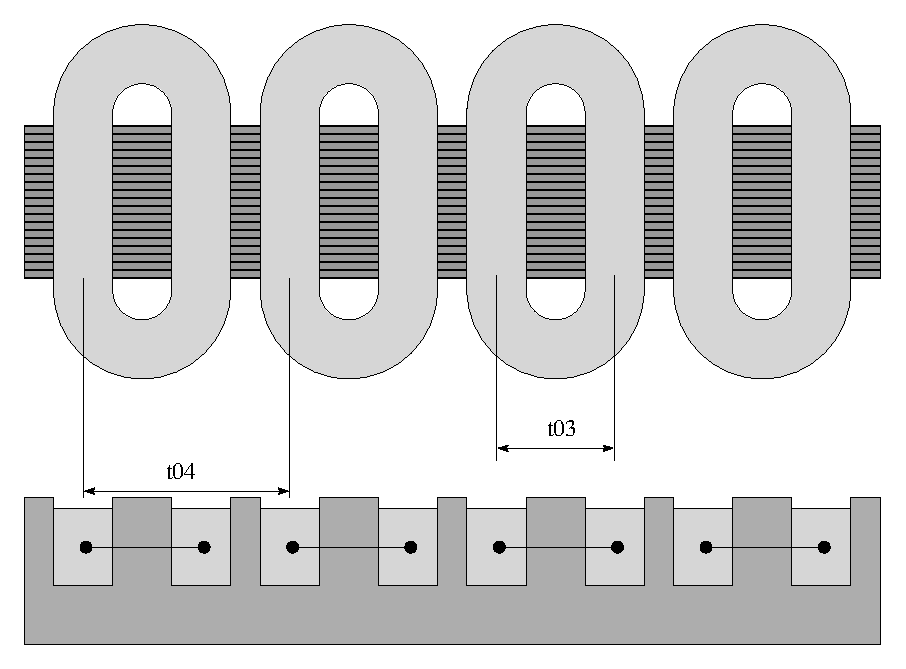
\includegraphics[width=0.42\textwidth]{figs/f_concen_coils-a.eps}
\end{psfrags}%}
  \hfill
  \subfloat[Double layer\label{fig:concen-b}]{
  \begin{psfrags}%
\psfragscanon

% text strings:
\psfrag{t01}[bc]{(a) Single layer}
\psfrag{t02}[bc]{(b) Double layer}
\psfrag{t03}[bc]{$x \tau_s$}
\psfrag{t04}[bc]{$2\tau_s$}
\psfrag{t05}[bc]{$\tau_s$}

% Figure:
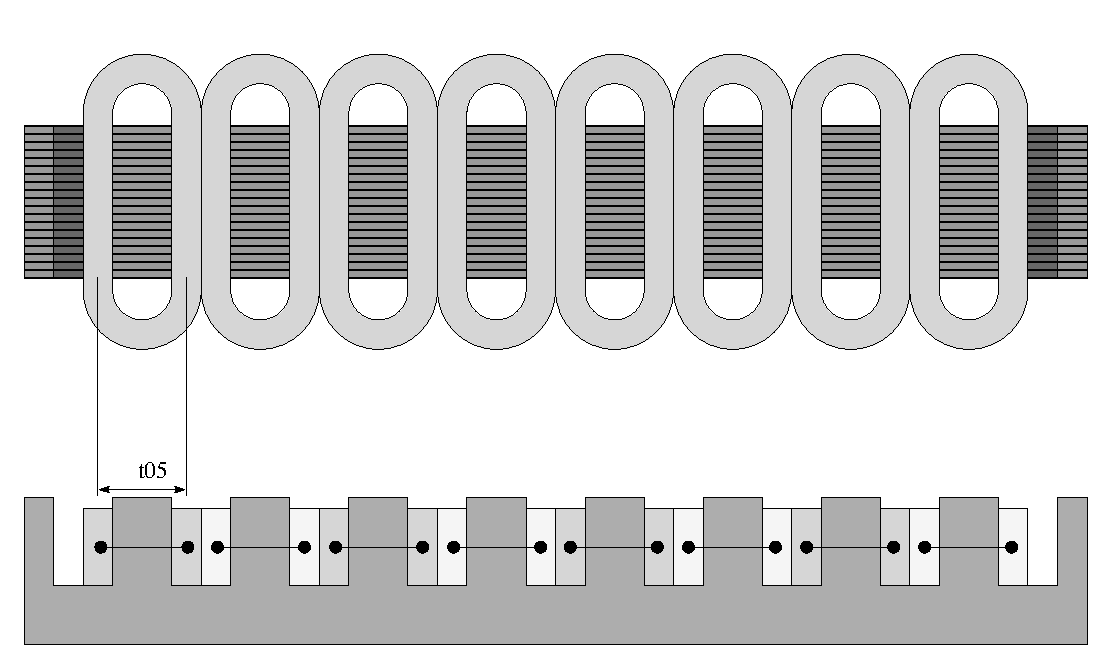
\includegraphics[width=0.52\textwidth]{figs/f_concen_coils-b.eps}
\end{psfrags}%}
  \caption{Single and double layer non-overlapping windings}
  \label{fig:concen_coils}
\end{figure}
\index{Zahnspulen}
\index{double layer}
\index{concentrated coils}
\index{tooth coils}

In the literature different definitions of terms are in use for non-overlapping concentrated windings. The most common of them are:
(a) concentrated windings \cite{REF-00822}; (b) concentrated fractional pitch windings \cite{REF-00823};  (c) fractional slot wound \cite{REF-00815}; and (d) fractional slot \cite{REF-01044}.

If the coils are to be equally in shape, which simplifies manufacturing, it is recognised that a single layer could easily have a variable slot pitch\footnote{The concept of a variable coil pitch is shown in Fig.~\ref{fig:f_slotstar}.} Furthermore, the coils could be implemented as either form-wound or round-wound. Returning to the variable coil pitch of the single layer, it is important to mention that this is an extra degree of freedom that offers to be an attractive design parameter. The air gap flux that links the coil could thus be increased and torque ripple can be improved. 
\index{regular}
\index{irregular}
\index{form-wound}
\index{round-wound}

It is therefore helpful to classify a concentrated winding either as an overlapping or non-overlapping concentrated winding. Reference \cite{REF-00754} certainly aroused interest in non-overlapping concentrated windings with their paper entitled ``Synthesis of High Performance PM Motors With Concentrated Windings'', since this is a paper which is very often used as a reference on these winding types. This could be a possible explanation for the use of the term ``concentrated windings'' rather than ``tooth coil windings''.

The expansion of the classical winding types used in machines by non-overlapping windings offers new possibilities in especially traction machine design. The main research question in section \ref{sec:problem_statement} suggests a design algorithm that takes into account the non-overlapping type. Obviously a method that is valid for all types is required. In addition, it should be easy to integrate into whichever process is in use.

\section{Notes to the reader}
The work presented in this thesis was done in N\"urnberg, Germany. Consequently many of the literature used were in German. To name only a few, books by \cite{REF-00004}, \cite{REF-00429} and \cite{REF-00294} are still commonly used in design offices. It is noticeable that even though there exists a list of symbols for various quantities, English and German have in some cases different symbols for the same quantity. This is mainly due to the fact that languages develop individual and of course colloquial language rules. Even a direct translation does not necessarily give the typical word used. An example is the German word \textit{Felderregerkurve}. A direct translation would be ``field excitation curve'', which of course is not wrong. However, the field excitation curve in electrical terms is usually known as the ``magnetomotive force'' (mmf). Tab.~\ref{tab:translation} gives some common electrical machine quantities in English and German, and the different symbols in use.
\begin{table}[htbp]
  \caption[Typical machine quantities and their German translation]%
  {Typical machine quantities, and their German counterparts}
  \label{tab:translation}
  \centering
  \begin{tabular}{lccl}
  \toprule
  Quantity   &  English  & German & Unit \\
  \toprule
  magnetomotive force (\textit{Durchflutung}) & 
  $F$& $\Theta$ & \SI{}{A}\\
  \midrule
  flux linkage (\textit{Flussverkettung}) & 
  $\lambda$& $\psi$ & \SI{}{V.s}   \\
  \midrule
  voltage (\textit{Spannung})  & 
  $V$& $U$ & \SI{}{V} \\
  \midrule
  specific resistance (\textit{spezifischer Widerstand})&
  $\rho$& $\varrho$ & \SI{}{\ohm.m} \\
  \midrule
  specific weight (\textit{spezifischer Masse})&
  $\rho$& $\gamma$& \SI{}{kg.m^{-3}}\\
  \midrule
  conductivity (\textit{Leitf\"ahigkeit})&
  $\sigma$&$\kappa$& \SI{}{S.m^{-1}}\\
  \midrule
  cross section area (\textit{Querschnitt})&
  $A$&$Q$& \SI{}{m^{2}}\\
  \midrule
  turn number (\textit{Windungszahl}) & 
  N& W & - \\
  \bottomrule
  \end{tabular}
\end{table}
\index{magnetomotive force}
\index{flux linkage}
\index{turn number}
\index{specific resistance}
\index{specific weight}
\index{Felderregerkurve}

It is commendable that the German terminology on electrical machines allows a very precise description of almost all aspects related to the subject. In many cases it is difficult to find an equivalent technical term in English, because it simply does not exist. The problem of different terminologies even exists within a language: different ``schools'' use different terms which makes the study of machine related books not easy. Also historical changes need to be kept in mind.

%The term ``machine'' is preferred throughout the book  and means it could be a machine that is operated either as a motor or as a generator. In the title the term ``motor'' is used, since only the measured results of motor operation are presented. However, in the theoretical sections, the word ``machine'' is preferred. 
%\index{machine}
%\index{motor} 

The discrete Fourier transform (DFT) has much in common with the winding factor and its definition is given in \eqref{eqn:DFTdef}. Note that the exponent is a negative number and complex. The reason for the negative exponent is explained in \cite{REF-01048,REF-01049,REF-01050}. For the complex notation a $\i$ and not a $i$ is used. Furthermore, to keep the equations compact the complex exponent will be written as $e^z$ rather than $e^{-\i\theta}$.
\begin{equation}\label{eqn:DFTdef}
  X(k)=\sum_{j=1}^{N}x(j)e^z
  \qquad
  \begin{cases}
    j \in \left\{1,\ldots,N  \right\} \rightarrow \; \mbox{sampled data}\\
  	k \in \left\{1,\ldots,N  \right\} \rightarrow \; \mbox{harmonic order}\\
    z = -\i\theta   \\
  	\theta = \frac{2\pi}{N}   \\
  	e^{-\theta \i} = \cos (-\theta) + \i \sin (-\theta)
  \end{cases}
\end{equation}
An important difference between the complex winding factor and the DFT is the phase information. In a typical DFT it is assumed that the sampled points are equidistant, i.e.~$\frac{2\pi}{N}$. The geometrical position of the stator slots around the air gap peripheral is the phase information. Through the phase information it is thus possible to calculate the winding factors for non equidistant stator slots. 

\section{Design program}
A Matlab script that implements the algorithm in Fig.~\ref{fig:flowchart} is used to plot the examples given in Tab.~\ref{tab:Example_table}. The complete program listings are given in \ref{sec:malg} and \ref{sec:mex}. Start the script by typing from the Matlab promt:

\begin{lstlisting}[language=matlab]
wnd = arun(1);
\end{lstlisting}
The resulting plots are shown in Fig.~\ref{fig:tests} and the Matlab code is provided in appendix \ref{sec:mex}.

